Drone cameras are everywhere.
In the last few years, these devices have emerged as a fundamentally new kind of consumer camera.
Indeed, the US government forecasts that over 3 million consumer drones will be deployed nationally by 2019 \cite{faa:2017}.
The rapidly growing popularity of drone cameras can be attributed to their small size, low cost, and unprecedented agility.
Drone cameras can maneuver through their environment in a totally freeform way, and there is an exciting and dynamic quality to drone footage that is nearly impossible to obtain otherwise.\footnote{As an example of particularly compelling drone footage, we encourage the reader to watch this shot of Venice Beach by Robert McIntosh, one of the world's best drone pilots: \url{https://vimeo.com/218839072}.}

In particular, drone cameras are enabling professional filmmakers to tell stories in new ways. 
For example, drones are being used to film scenes in a growing number of Hollywood movies, including \textsc{The Wolf of Wall Street}, \textsc{Transformers}, and \textsc{Skyfall} \cite{nyt:2014,wsj:2015}.
But the potential applications for drone cameras extend far beyond Hollywood.
Drone cameras are being used in disaster relief scenarios \cite{michael:2012}, wildlife monitoring \cite{duke:2017}, journalism \cite{indivisible:2017}, 3D mapping \cite{pix4d:2015}, surveying \cite{3dr:2017a}, and inspection \cite{alexis:2015}.

But drone cameras are hard to use.
It is challenging for novice users to fly simple trajectories without crashing, and it is challenging for experts to obtain the kind of smooth and aesthetically pleasing footage you'd expect to see in a Hollywood movie.

\begin{tcolorbox}[before skip=20pt, after skip=20pt, sharp corners]
\begin{center}
\textbf{Our ultimate goal in this dissertation is to make drone cameras easier to use.}
\end{center}
\end{tcolorbox}

\section{Why Are Drone Cameras Hard To Use?}


\begin{figure*}[th!]
\centering
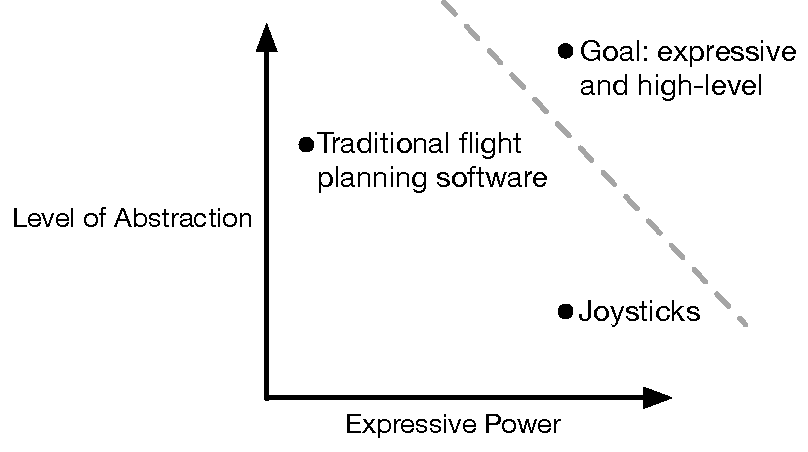
\includegraphics[width=4.0in]{images/2018_introduction/intro.pdf}
\caption{
Overview of existing user interfaces for drone camera systems.
On the one hand, joysticks are highly expressive but too low-level.
On the other hand, traditional flight planning software is high-level but not expressive enough.
Our goal in this dissertation is to build drone camera systems that are expressive and high-level.
}
\label{fig:ch1:intro}
\end{figure*}

Today, the most common method for practitioners to control drone cameras is to pilot them manually with remote-control joysticks.
Joysticks are \emph{expressive}, in the sense that experts can use joysticks to express an incredibly wide range of drone motion.
But joysticks can be counter-intuitive for novice users, because the user must translate high-level goals for the drone (e.g., ``get low to the ground and go towards that building") into low-level joystick movements (e.g., ``pull back on the left joystick and simultaneously sweep towards 12 o'clock on the right joystick).
This task is especially demanding because joystick commands typically correspond to drone actions in the \emph{body frame} of the drone (i.e., the coordinate system that is rigidly attached to the drone). 
For example, pressing up on a joystick will move the drone forward in the body frame.
But high-level user goals are typically easier to express in the \emph{world frame} (i.e., the coordinate system that is rigidly attached to the environment).

When filming with a drone, users must also control the orientation of the camera, which is typically mounted on an independently controlled joint known as a \emph{gimbal}.
It is especially challenging to control the gimbal while simultaneously maneuvering the drone.
With this difficulty in mind, expert pilots often work in teams, with one pilot controlling the drone motion, and another controlling the gimbal.

As an alternative to flying with joysticks, flight planning software has been developed to control a drone by specifying GPS waypoints on a 2D map. 
The user is responsible for setting waypoints before a flight, and the drone subsequently flies in auto-pilot mode and attemps to follow the waypoints.
This type of flight planning software is \emph{high-level}, in the sense that it does not require the user to explicitly specify moment-to-moment navigation commands for the drone.
But existing flight planning software is not expressive enough.
There are many interesting maneuvers that a drone could safely execute, that are difficult or impossible to express in existing flight planning software.

Figure \ref{fig:ch1:intro} summarizes the landscape of existing user interfaces for drone cameras.
On the one hand, joysticks are highly expressive but too low-level.
On the other hand, existing flight planning software is high-level but not expressive enough.
In order for drone cameras to become widely adopted by non-expert pilots (e.g., journalists, fire fighters, biologists, real-estate agents, indie filmmakers, etc.), we need user interfaces that are both expressive and high-level.
In other words, we need interfaces that expose a wide range of drone maneuvers to the user, while also making it easy to specify high-level goals and desired behaviors.

\section{Why Do We Need Trajectory Optimization?}

It is fundamentally challenging to build user interfaces for drone cameras that are expressive and high-level.
As our user interfaces move away from explicitly specifying motor torques, computing the final intended drone trajectory from the user's input becomes increasingly \emph{ambiguous}.
The underlying computational problems become increasingly \emph{ill-posed}.
If we want to build high-level interfaces that are useful for non-experts, we must somehow decide how to interpret the ambiguous input we will get from the user.

\begin{tcolorbox}[before skip=20pt, after skip=20pt, sharp corners]
\begin{center}
\textbf{The big idea in this dissertation is to use the principles of \emph{trajectory optimization} to recover a user's intended drone trajectory, given some high-level description from a user.}
\end{center}
\end{tcolorbox}

\noindent In this dissertation, we will be formulating trajectory optimization problems, where we want to somehow choose a sequence of drone actions to minimize some cost function subject to some constraints, e.g.,
~
\begin{equation*}
\begin{aligned}
& \text{choose drone actions } \mathbf{u}_1, \mathbf{u}_2, \ldots, \mathbf{u}_T\\
& \text{to minimize a cost function } \sum_{t=1}^T c( \mathbf{x}_t, \mathbf{u}_t)\\
& \text{subject to user constraints and drone constraints}
\end{aligned}
\end{equation*}

\noindent where $\mathbf{x}_1, \mathbf{x}_2, \ldots, \mathbf{x}_T$ is the sequence of drone states corresponding to the sequence of drone actions.
The cost functions we choose are going to depend on the particular application domain, and will vary as we progress through the dissertation.
Our cost functions are going to encode things like user preferences, as well as any prior knowledge we have about a particular application domain.
Our constraints are going to encode things like strict user requirements, as well as our drone's physical limits.

Trajectory optimization problems of this form are not new, and the corresponding solution methods have been widely applied to drones \cite{kumar:2012}.
But they have not been widely applied to drone cameras.
In this dissertation, we will apply the principles of trajectory optimization to drone cameras in new ways.
We will use domain knowledge that is specialized to a particular drone camera task, and we will reformulate classical trajectory optimization problems in terms of the drone camera's visual output, i.e., in terms of what the drone is \emph{seeing}.
We will apply this methodology in two distinct application domains: drone cinematography and drone 3D scanning.
In doing so, we will take several steps towards our ultimate goal of making drone cameras easier to use and more expressive.

\section{Dissertation Overview and Summary of Contributions}

\begin{figure*}[t!]
\centering
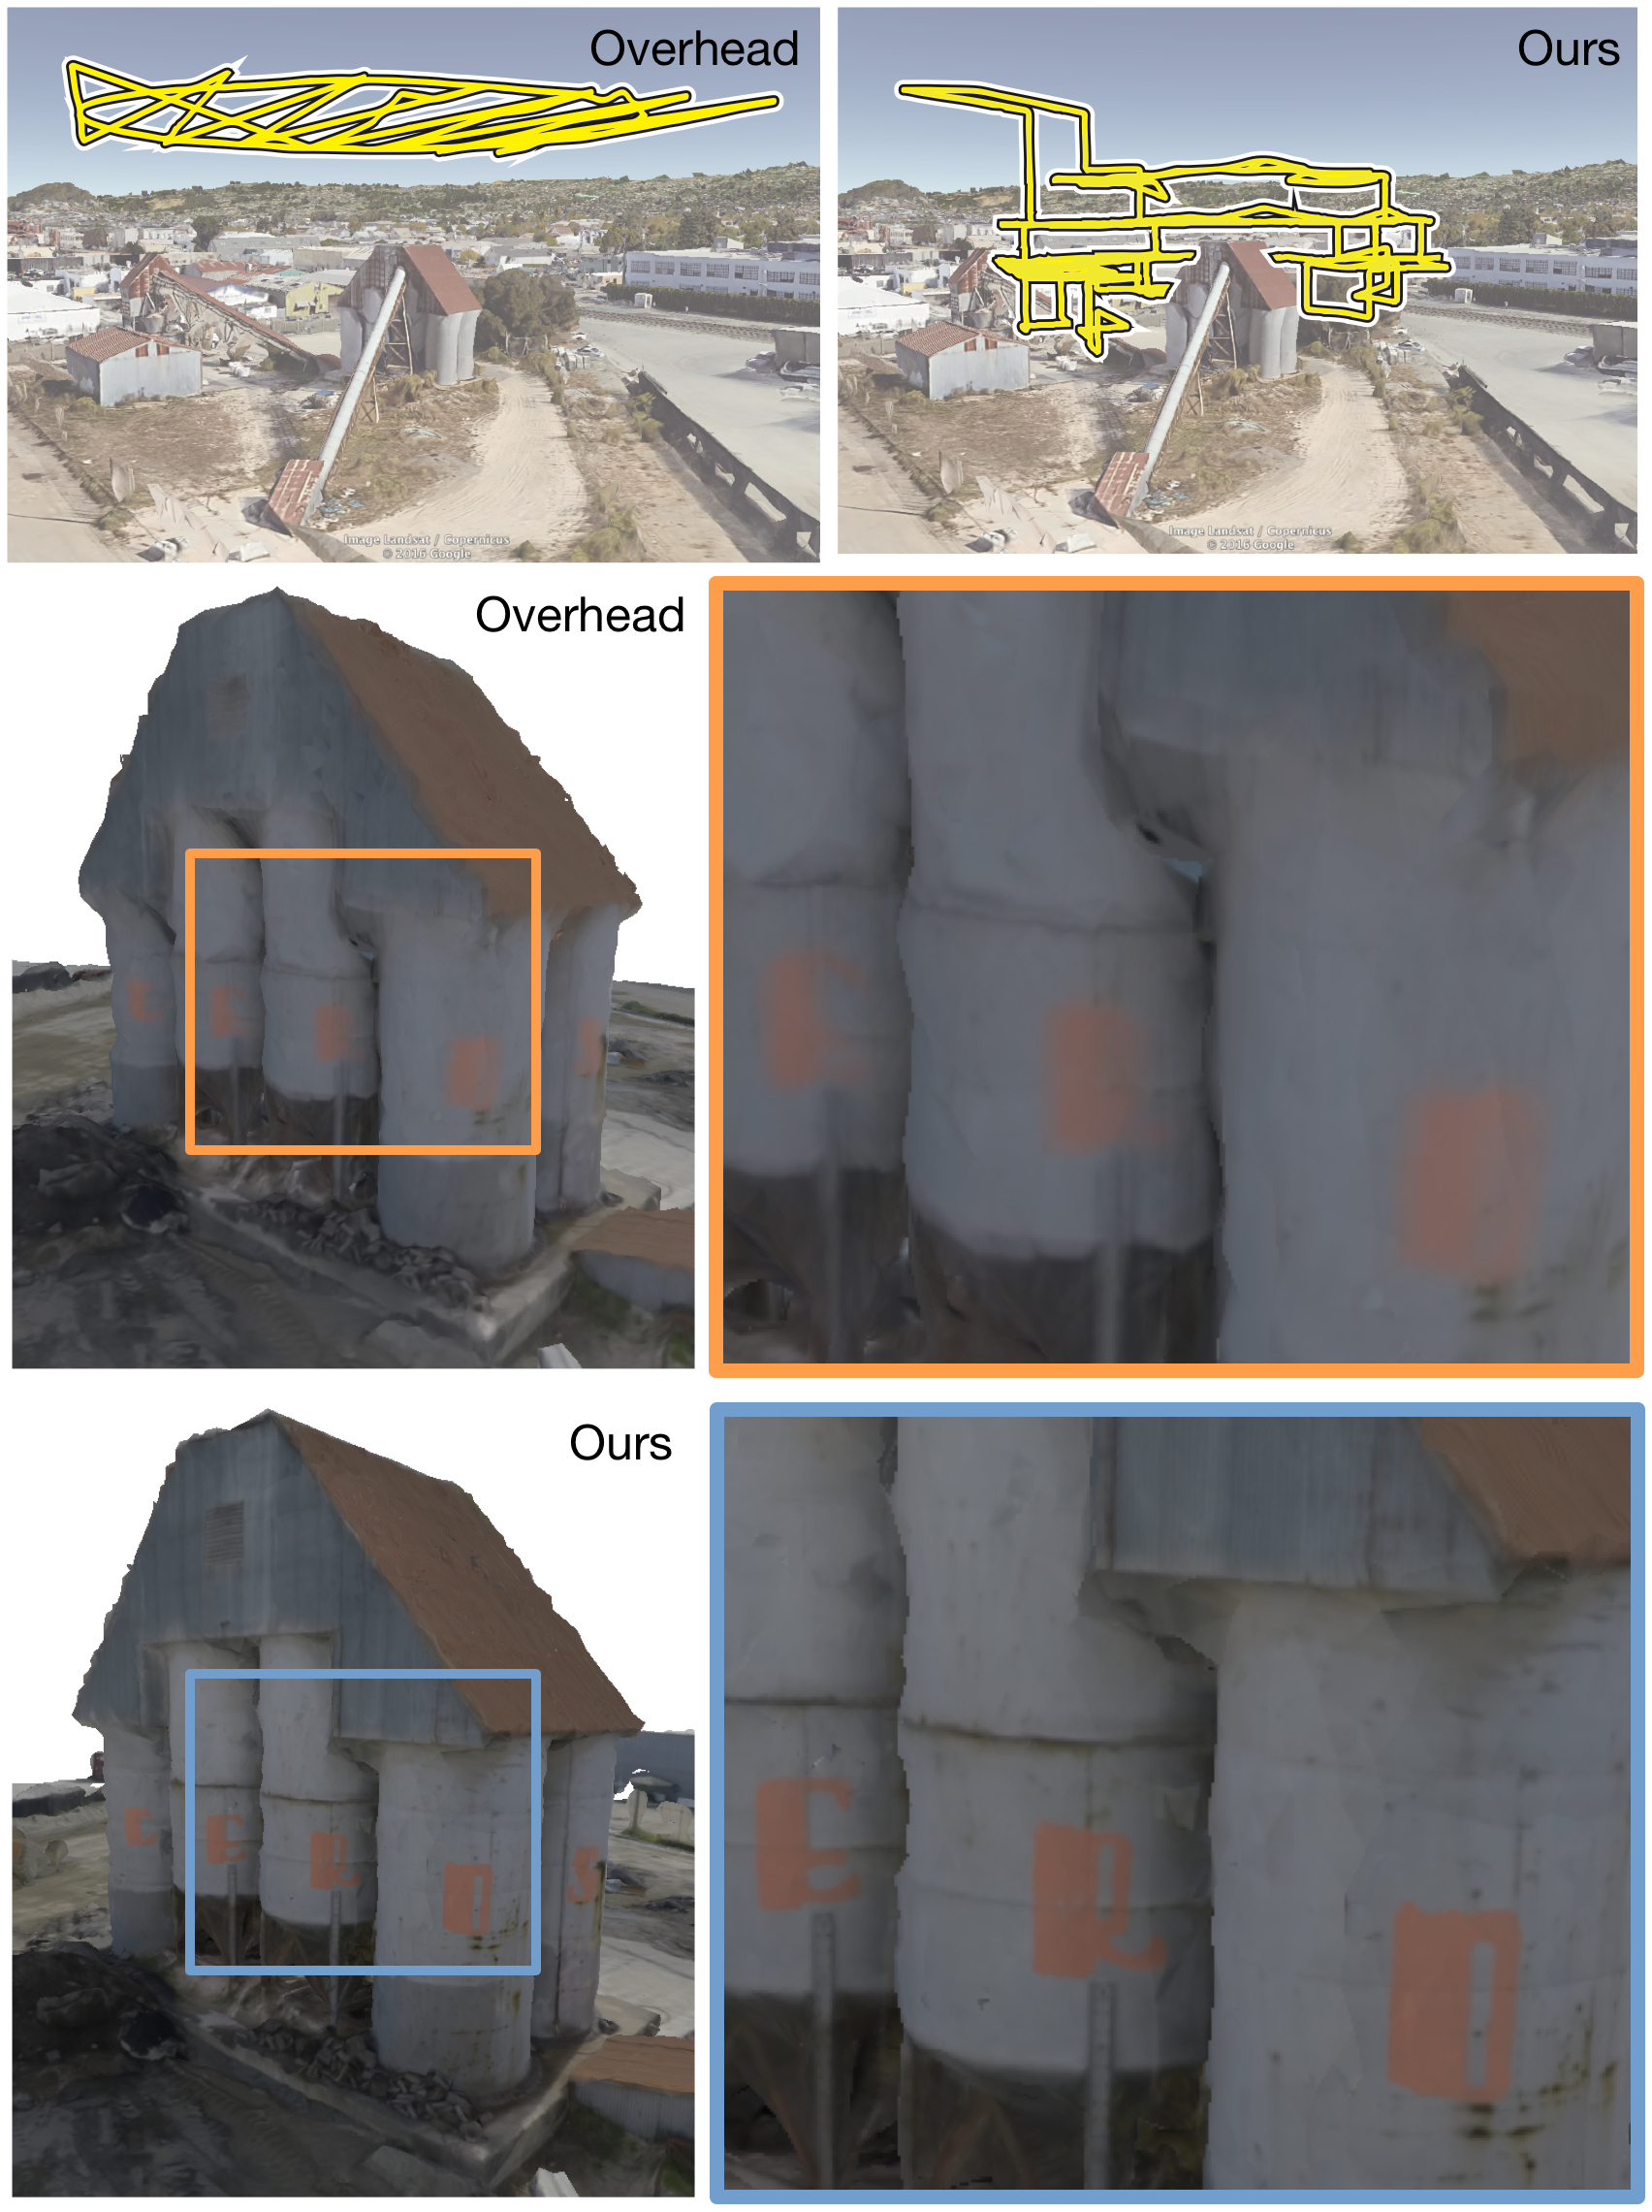
\includegraphics[width=6.0in]{images/2015_siggraph_asia/teaser.pdf}
\caption{
(Left) Our interactive tool for designing quadrotor camera shots.
In our tool, users specify camera pose keyframes in a virtual environment using a 3D scene view (a) and a 2D map view (b).
Our tool synthesizes a camera trajectory that obeys the physical equations of motion for quadrotors, and interpolates between the user-specified keyframes.
Users can preview the resulting shot in the virtual environment, using the playback buttons and scrubber interface to navigate through the shot (c).
Users can also control the precise timing of the shot by editing easing curves (d).
Users can set the virtual camera's field of view to match their real-world camera (e).
Our tool provides the user with visual feedback about the physical feasibility of the resulting trajectory, notifying the user if her intended trajectory violates the physical limits of her quadrotor hardware (f).
Once the user is satisfied with her shot, she presses the Start Capture button (g).
(Right) Our tool commands a quadrotor camera to execute the resulting trajectory fully autonomously, capturing real video footage that is faithful to the virtual preview.
We show frames from our real-world video output, with corresponding frames from the virtual preview shown as small insets (h).
We provide an overview of our tool at \url{http://youtu.be/Ds-KF4ZSnAo}.
}
\label{fig:ch1:teaser_ch2}
\end{figure*}

\begin{figure*}[t!]
\centering
\includegraphics[width=6.0in]{images/2016_siggraph/06_teaser.pdf}
\caption{
Our algorithm for generating feasible quadrotor camera trajectories.
Our algorithm takes as input an infeasible quadrotor camera trajectory (top row, left) and produces as output a feasible trajectory that is as similar as possible to the input trajectory (top row, right).
By design, our algorithm does not change the spatial layout or  visual contents of the input trajectory.
Instead, our algorithm guarantees the feasibility of the output trajectory by re-timing the input trajectory, perturbing its timing as little as possible while remaining within velocity and control force limits (top row, insets).
Our algorithm runs at interactive rates, solving for the feasible trajectory shown above in less than 2 seconds.
Infeasible trajectories can be unsafe to fly on real quadrotor cameras, but we can safely fly the feasible trajectories generated by our algorithm, producing real video footage that is faithful to a \textsc{Google Earth} shot preview (bottom row).
We provide an overview of our algorithm at \url{http://youtu.be/zhik1D2o6Fc}.
}
\label{fig:ch1:teaser_ch3}
\end{figure*}


\begin{figure}[t!]
\begin{center}
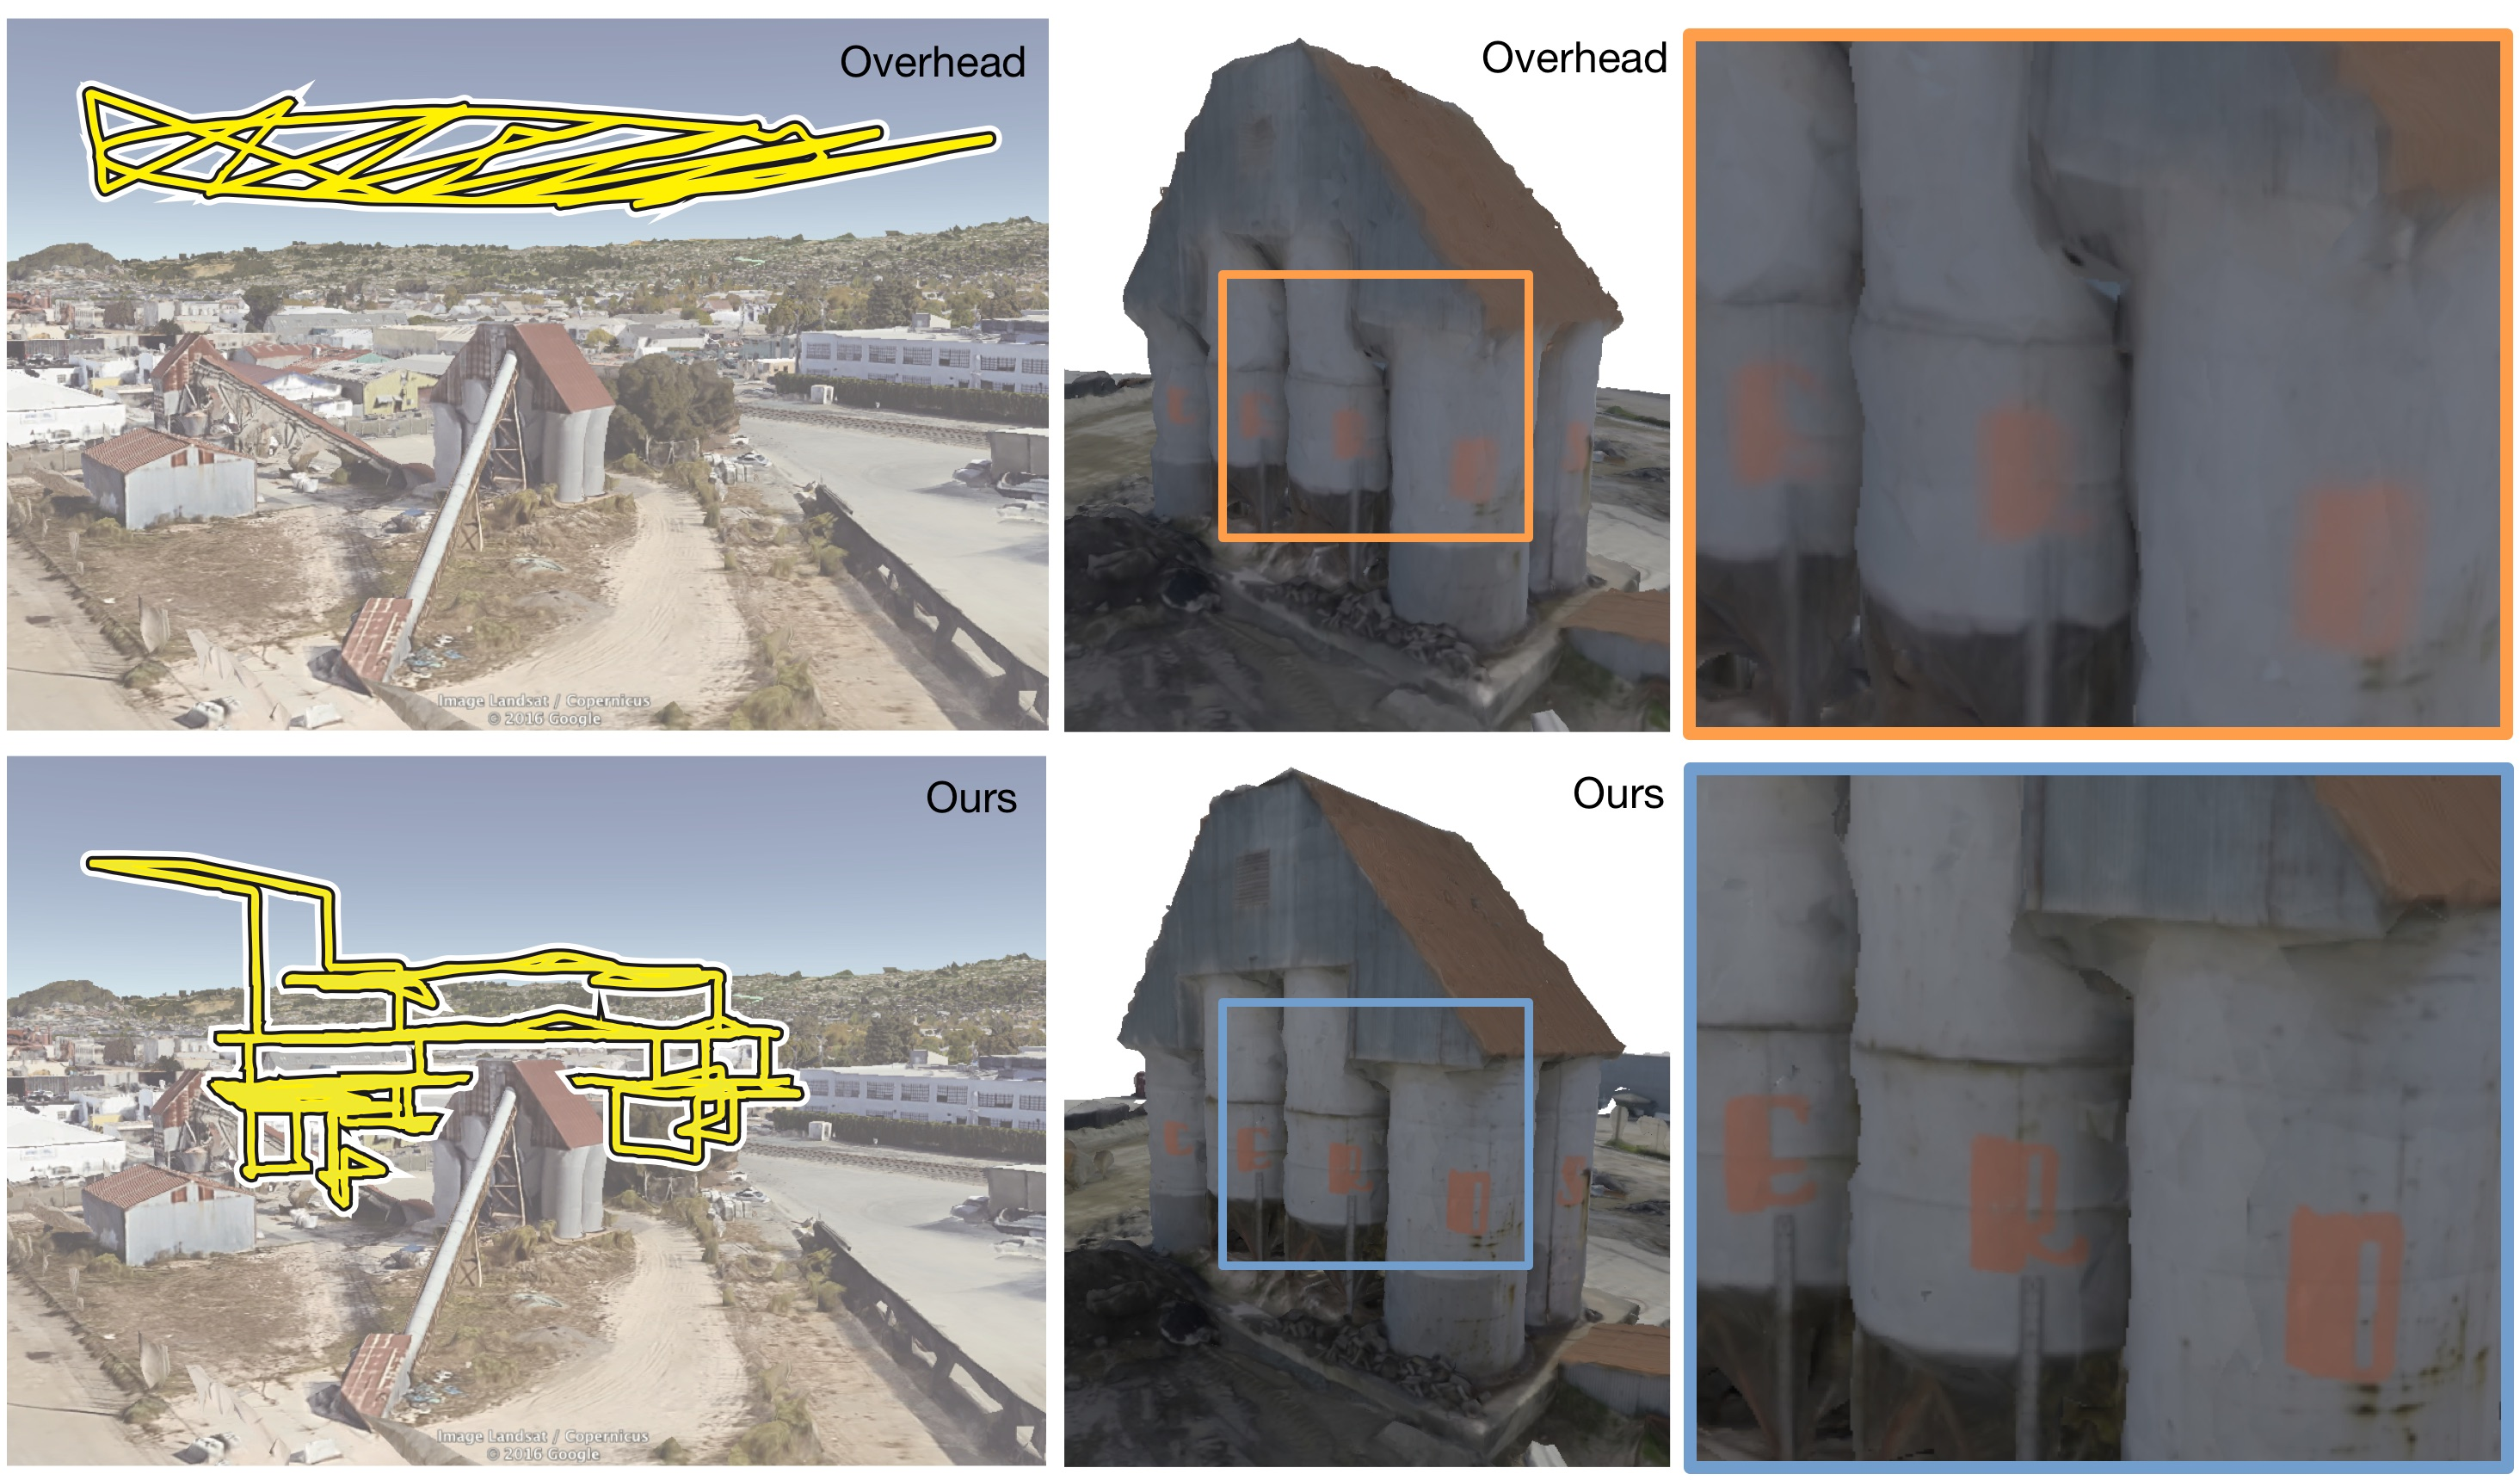
\includegraphics[width=6.0in]{images/2017_iccv/teaser_web.pdf}
\end{center}
\caption{
3D reconstruction results obtained using our algorithm for generating aerial 3D scanning trajectories, as compared to an overhead trajectory.
Left column: Google Earth visualizations of the trajectories.
Middle and right columns: results obtained by flying a drone along each trajectory, capturing images, and feeding the images to multi-view stereo software.
Our trajectories lead to noticeably more detailed 3D reconstructions than overhead trajectories.
In all our experiments, we control for the flight time, battery consumption, number of images, and quality settings used in the 3D reconstruction.
We provide an overview of our algorithm at \url{http://youtu.be/89fFmfVZSO8}.
}
\label{fig:ch1:teaser_ch4}
\end{figure}

\begin{table}[t]
\centering
\footnotesize
\begin{tabular}{@{}ll@{}}
\toprule
\multicolumn{2}{l}{ \textbf{An Interactive Tool for Designing Quadrotor Camera Shots (Chapter 2)} } \\
\midrule
Project page   & \url{http://stanford-gfx.github.io/Horus}         \\ 
Overview video & \url{http://youtu.be/Ds-KF4ZSnAo}                 \\  
Source code    & \url{http://github.com/stanford-gfx/Horus}        \\
               & \url{http://mikeroberts3000.github.io/flashlight} \\
\midrule
\multicolumn{2}{l}{ \textbf{Generating Dynamically Feasible Trajectories for Quadrotor Cameras (Chapter 3)} } \\
\midrule
Project page   & \url{http://graphics.stanford.edu/papers/feasible_trajectories} \\ 
Overview video & \url{http://youtu.be/zhik1D2o6Fc}                               \\  
Source code    & \url{http://mikeroberts3000.github.io/flashlight}               \\
\midrule
\multicolumn{2}{l}{ \textbf{Submodular Trajectory Optimization for Aerial 3D Scanning (Chapter 4)} } \\
\midrule
Project page   & \url{http://graphics.stanford.edu/papers/aerial_scanning} \\ 
Overview video & \url{http://youtu.be/89fFmfVZSO8}                         \\  
Source code    & \url{https://github.com/stanford-gfx/scanplan}            \\
\bottomrule
\end{tabular}
\normalsize
\caption{
Project pages, overview videos, and source code for each dissertation chapter.
}
\label{tbl:ch1:links}
\end{table}

In this dissertation, we make the following technical contributions.

\begin{itemize}

\item

In Chapter \ref{sec:ch2}, we introduce a software tool for designing and autonomously executing cinematography shots with quadrotor cameras (see Figure \ref{fig:ch1:teaser_ch2}).
Our tool enables users to: (1) specify shots visually using keyframes; (2) preview the resulting shots in a virtual environment; (3) precisely control the timing of shots using easing curves; and (4) capture the resulting shots in the real world with a single button click using a commercially available quadrotor camera.
We evaluate our tool in a user study with novice and expert cinematographers.
We show that our tool makes it possible for novices and experts to design compelling shots, and capture them fully autonomously.

\item 

To support our tool, we introduce a physical model for quadrotor cameras, in which a rigid body quadrotor is attached to a camera mounted on a gimbal.
We analyze the dynamics of our model, and show that camera trajectories must be $C^4$ continuous in order to obey the physical equations of motion for quadrotors.
With this requirement in mind, we derive an algorithm for synthesizing $C^4$ continuous camera trajectories from user-specified keyframes and easing curves.
This algorithm enables users to design shots visually, and gives users precise control over the timing of their shot.
We also derive an algorithm to compute the control signals required for a quadrotor and gimbal to follow any $C^4$ continuous camera trajectory.
This algorithm enables our tool to provide the user with visually accurate shot previews, and visual feedback about the physical feasibility of camera trajectories.

\item

In Chapter \ref{sec:ch3}, to further support our tool, we introduce a fast and user-friendly algorithm for generating camera trajectories that respect the dynamics and physical limits of quadrotor hardware (see Figure \ref{fig:ch1:teaser_ch3}).
We refer to such trajectories as being \emph{feasible}.
Our algorithm takes as input an infeasible camera trajectory designed by a user, and produces as output a feasible trajectory that is as similar as possible to the user's input.
By design, our algorithm does not change the spatial layout or  visual contents of the input trajectory.
Instead, our algorithm guarantees the feasibility of the output trajectory by \emph{re-timing} the input trajectory, perturbing its timing as little as possible while remaining within velocity and control force limits.
Our choice to perturb the timing of a shot, while leaving the spatial layout and visual contents of the shot intact, leads to a well-behaved non-convex optimization problem that can be solved at interactive rates.
We demonstrate that our algorithm is between 25$\times$ and 45$\times$ faster than a spacetime constraints approach implemented using a commercially available solver.
As we scale to more finely discretized trajectories, this performance gap widens, with our algorithm outperforming spacetime constraints by between 90$\times$ and 180$\times$.

\item

In Chapter \ref{sec:ch4}, we introduce an algorithm to generate drone camera trajectories, such that the imagery acquired during the flight will later produce a high-fidelity 3D model (see Figure \ref{fig:ch1:teaser_ch4}). Our method uses a coarse estimate of the scene geometry to plan camera trajectories that: (1) cover the scene as thoroughly as possible; (2) observe the scene geometry from a diverse set of viewing angles; (3) avoid obstacles; and (4) respect a user-specified flight time
budget. Our method relies on a mathematical model of scene coverage that exhibits an intuitive diminishing returns property known as \emph{submodularity}.
We leverage this property extensively to design a trajectory planning algorithm  that reasons globally about the non-additive coverage reward obtained across a trajectory, jointly with the cost of traveling between views.
We evaluate our method by using it to scan three large outdoor scenes, and we perform a quantitative evaluation using a photorealistic video game simulator.

\item

In Chapter \ref{sec:ch5}, we summarize our findings and discuss future research directions inspired by the preceding chapters.

\end{itemize}

\noindent Together, these contributions form a comprehensive toolbox of trajectory optimization methods for drone cameras.
In Table \ref{tbl:ch1:links}, we provide links to the project page, overview video, and open-source implementation for each chapter.
The overview videos are intended to be viewed before diving into each chapter.
This work appears in a series of previously published papers \cite{joubert:2015,roberts:2016,roberts:2017}.
The intended scope of the mathematical notation we introduce is local to each chapter, and related work is discussed within each chapter.
